\section{Tests}
\begin{frame}{Tests}
  Tests based on system responsiveness
  \begin{itemize}
    \item<1-> Docker vs VirtualBox startup
    \item<2-> SFC length startup 
  \end{itemize}

  \begin{textblock*}{5cm}(9cm, 2.5cm)
    
\includegraphics[scale=0.2]{test}
  \end{textblock*}
\end{frame}

% \subsection{Docker vs Hypervisor-based virtualization}
\begin{frame}{Tests - Docker vs VirtualBox}

  \begin{figure}
    \centering
    \begin{subfigure}[b]{0.35\textwidth}
      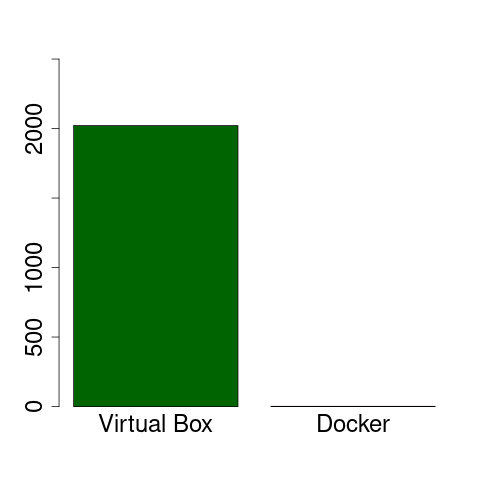
\includegraphics[width=\textwidth]{docker_vs_vmBarplotGraph}
    \end{subfigure}
    ~
    \begin{subfigure}[b]{0.35\textwidth}
      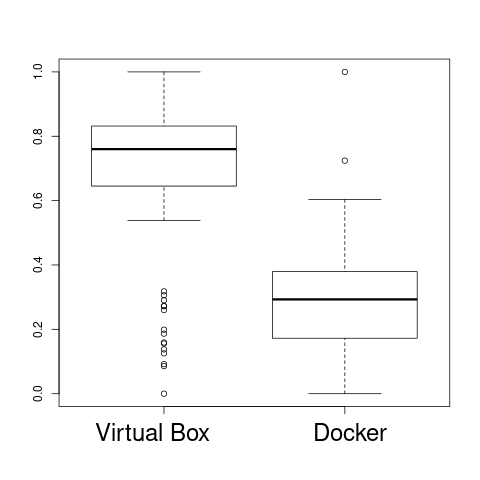
\includegraphics[width=\textwidth]{docker_vs_vmBoxplotGraph}
    \end{subfigure}
    \caption{Docker vs VirtualBox overall data sum comparison}
  \end{figure}

  \noindent $N = 100$ per technology

  \begin{itemize}
  \item Average start up time for Docker: 0.016 seconds
  \item Average start up time for Virtual Box: 20.211 seconds
  \end{itemize}

\end{frame}

% \subsection{SFC length startup}
\begin{frame}{Tests - SFC length startup}

  \begin{textblock*}{5cm}(8cm, 2cm)
    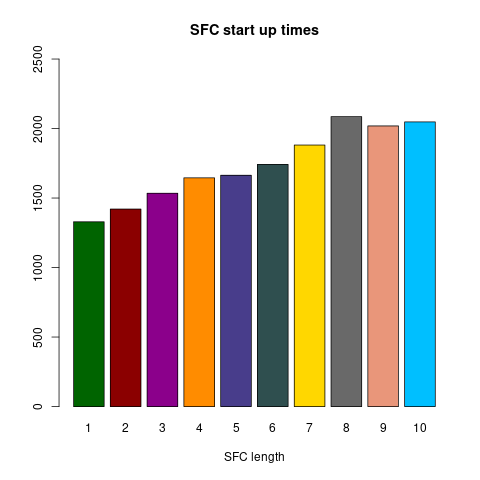
\includegraphics[scale=0.25]{sfc_startupBarplotGraph}
  \end{textblock*}

  \vspace*{1cm}

  \noindent $N = 100$ per SFC \newline

  \noindent Overhead due to
  \begin{itemize}
  \item Pod scheduling
  \item Resource allocation
  \item Route update
  \end{itemize}

  \vspace*{1cm}

  Average start up time (in seconds)
  \begin{multicols}{2}
    \begin{itemize}
    \item 1 element: 13.291 s
    \item 5 elements: 16.634 s
    \item 10 elements: 20.511 s
    \end{itemize}
  \end{multicols}

  \vfill
\end{frame}
